\section{Experiment}
% \begin{figure*}[t]
%   \centering
%   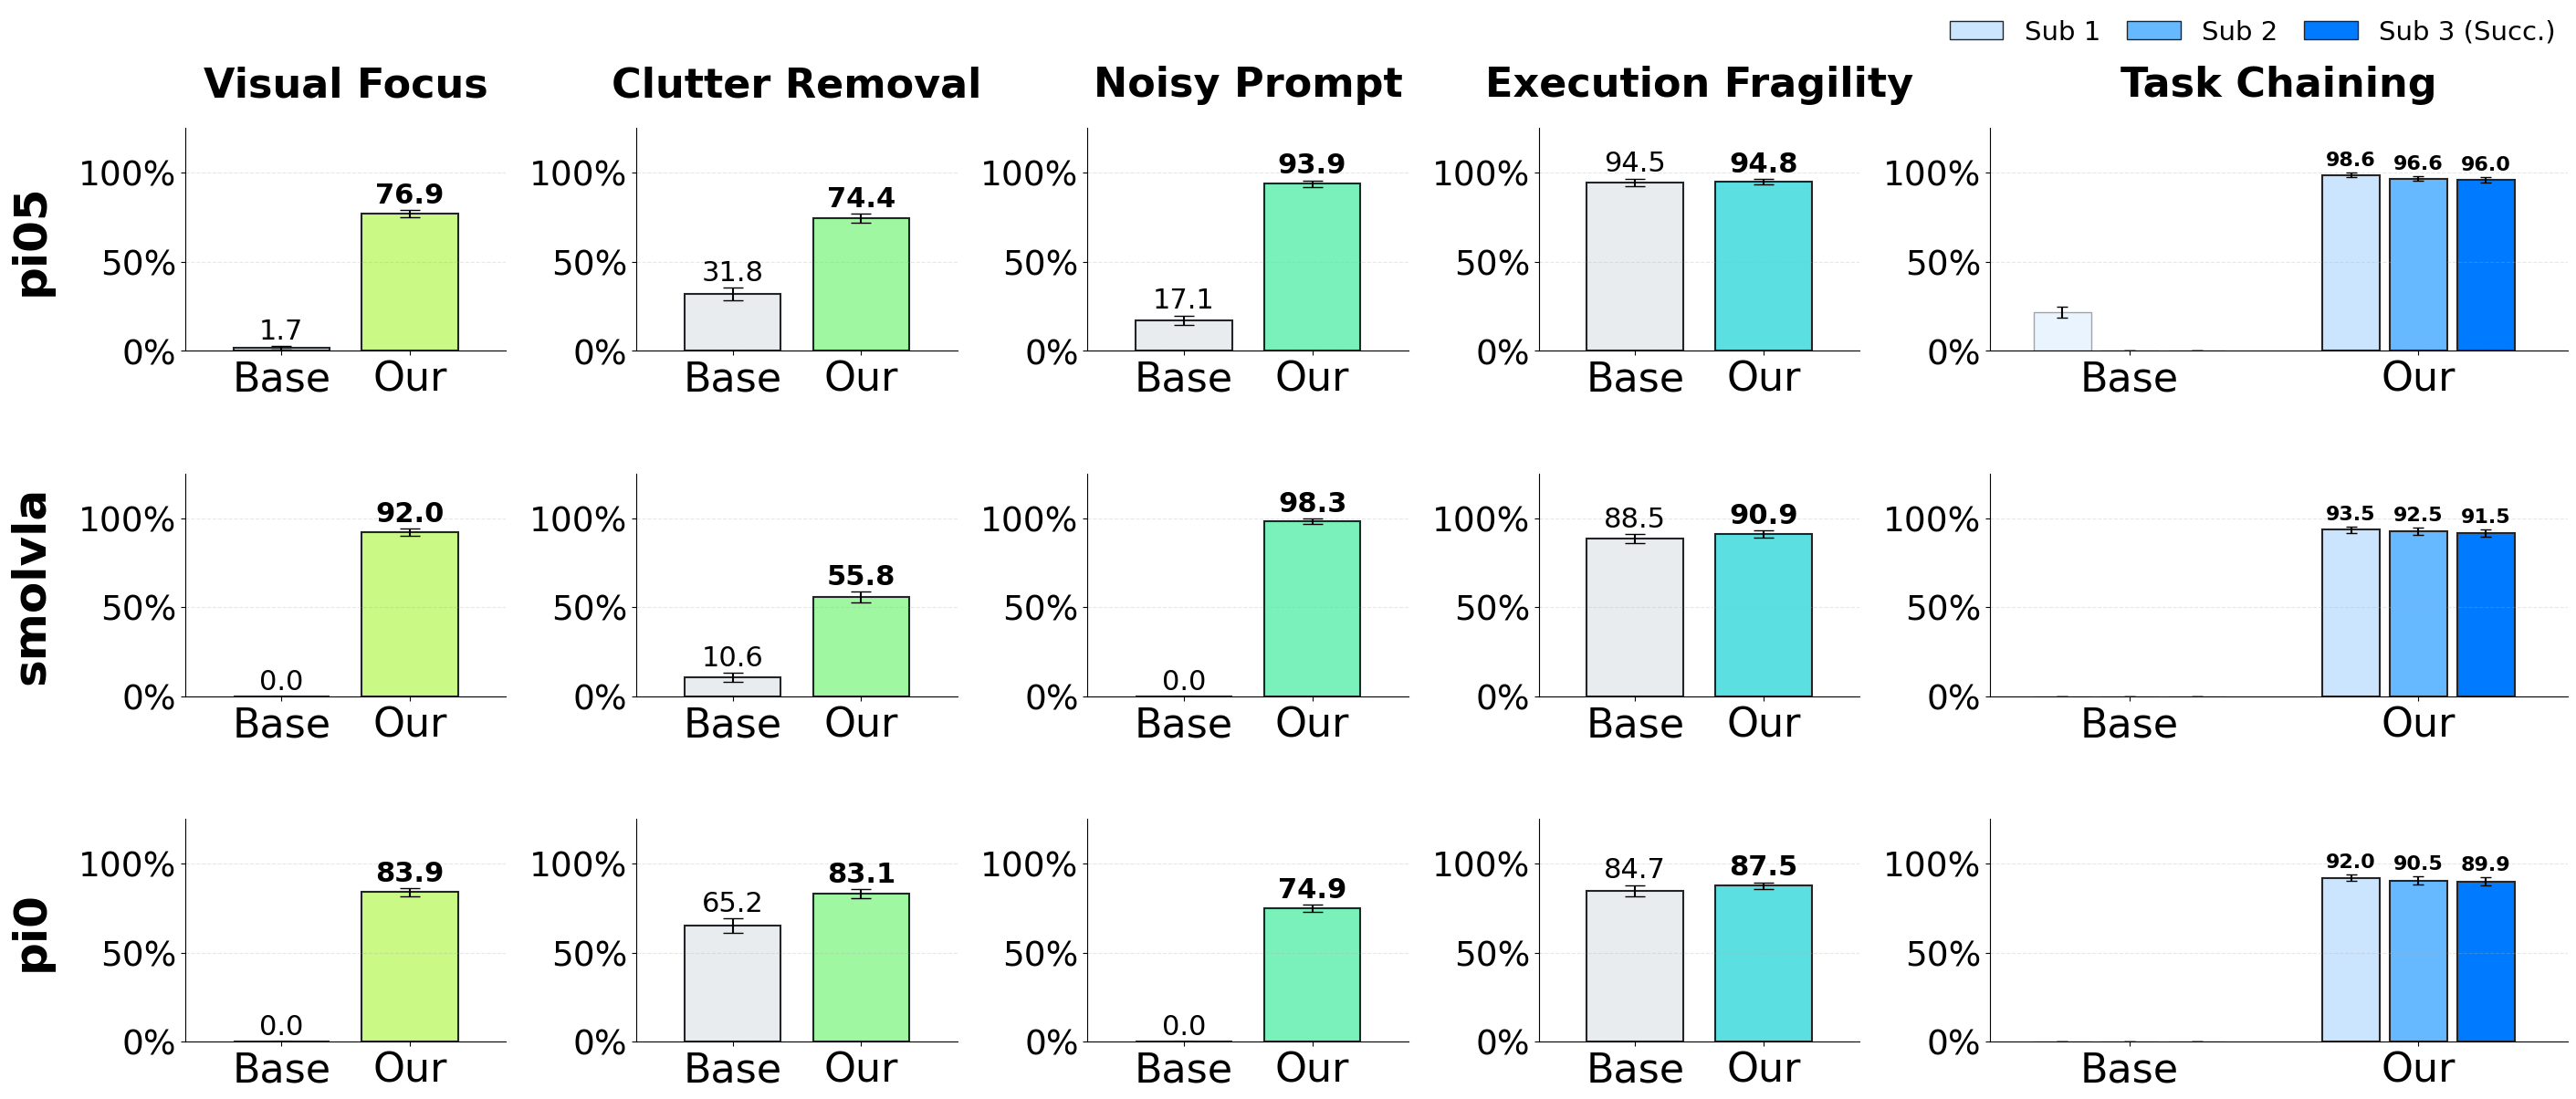
\includegraphics[width=0.95\linewidth]{figure/result.png}
%     \caption{\textbf{Performance comparison of {\sys} across diverse robotic foundation models and OOD challenges.} The results demonstrate that {\sys} consistently yields substantial performance gains for all base models across visual, linguistic, and long-horizon tasks.}%
%   \label{fig:result}
% \end{figure*}


\begin{figure*}[t]
  \centering
  \vspace{0.5em}
  \begin{minipage}[t]{0.66\textwidth}
    \vspace{0pt}
    \centering
    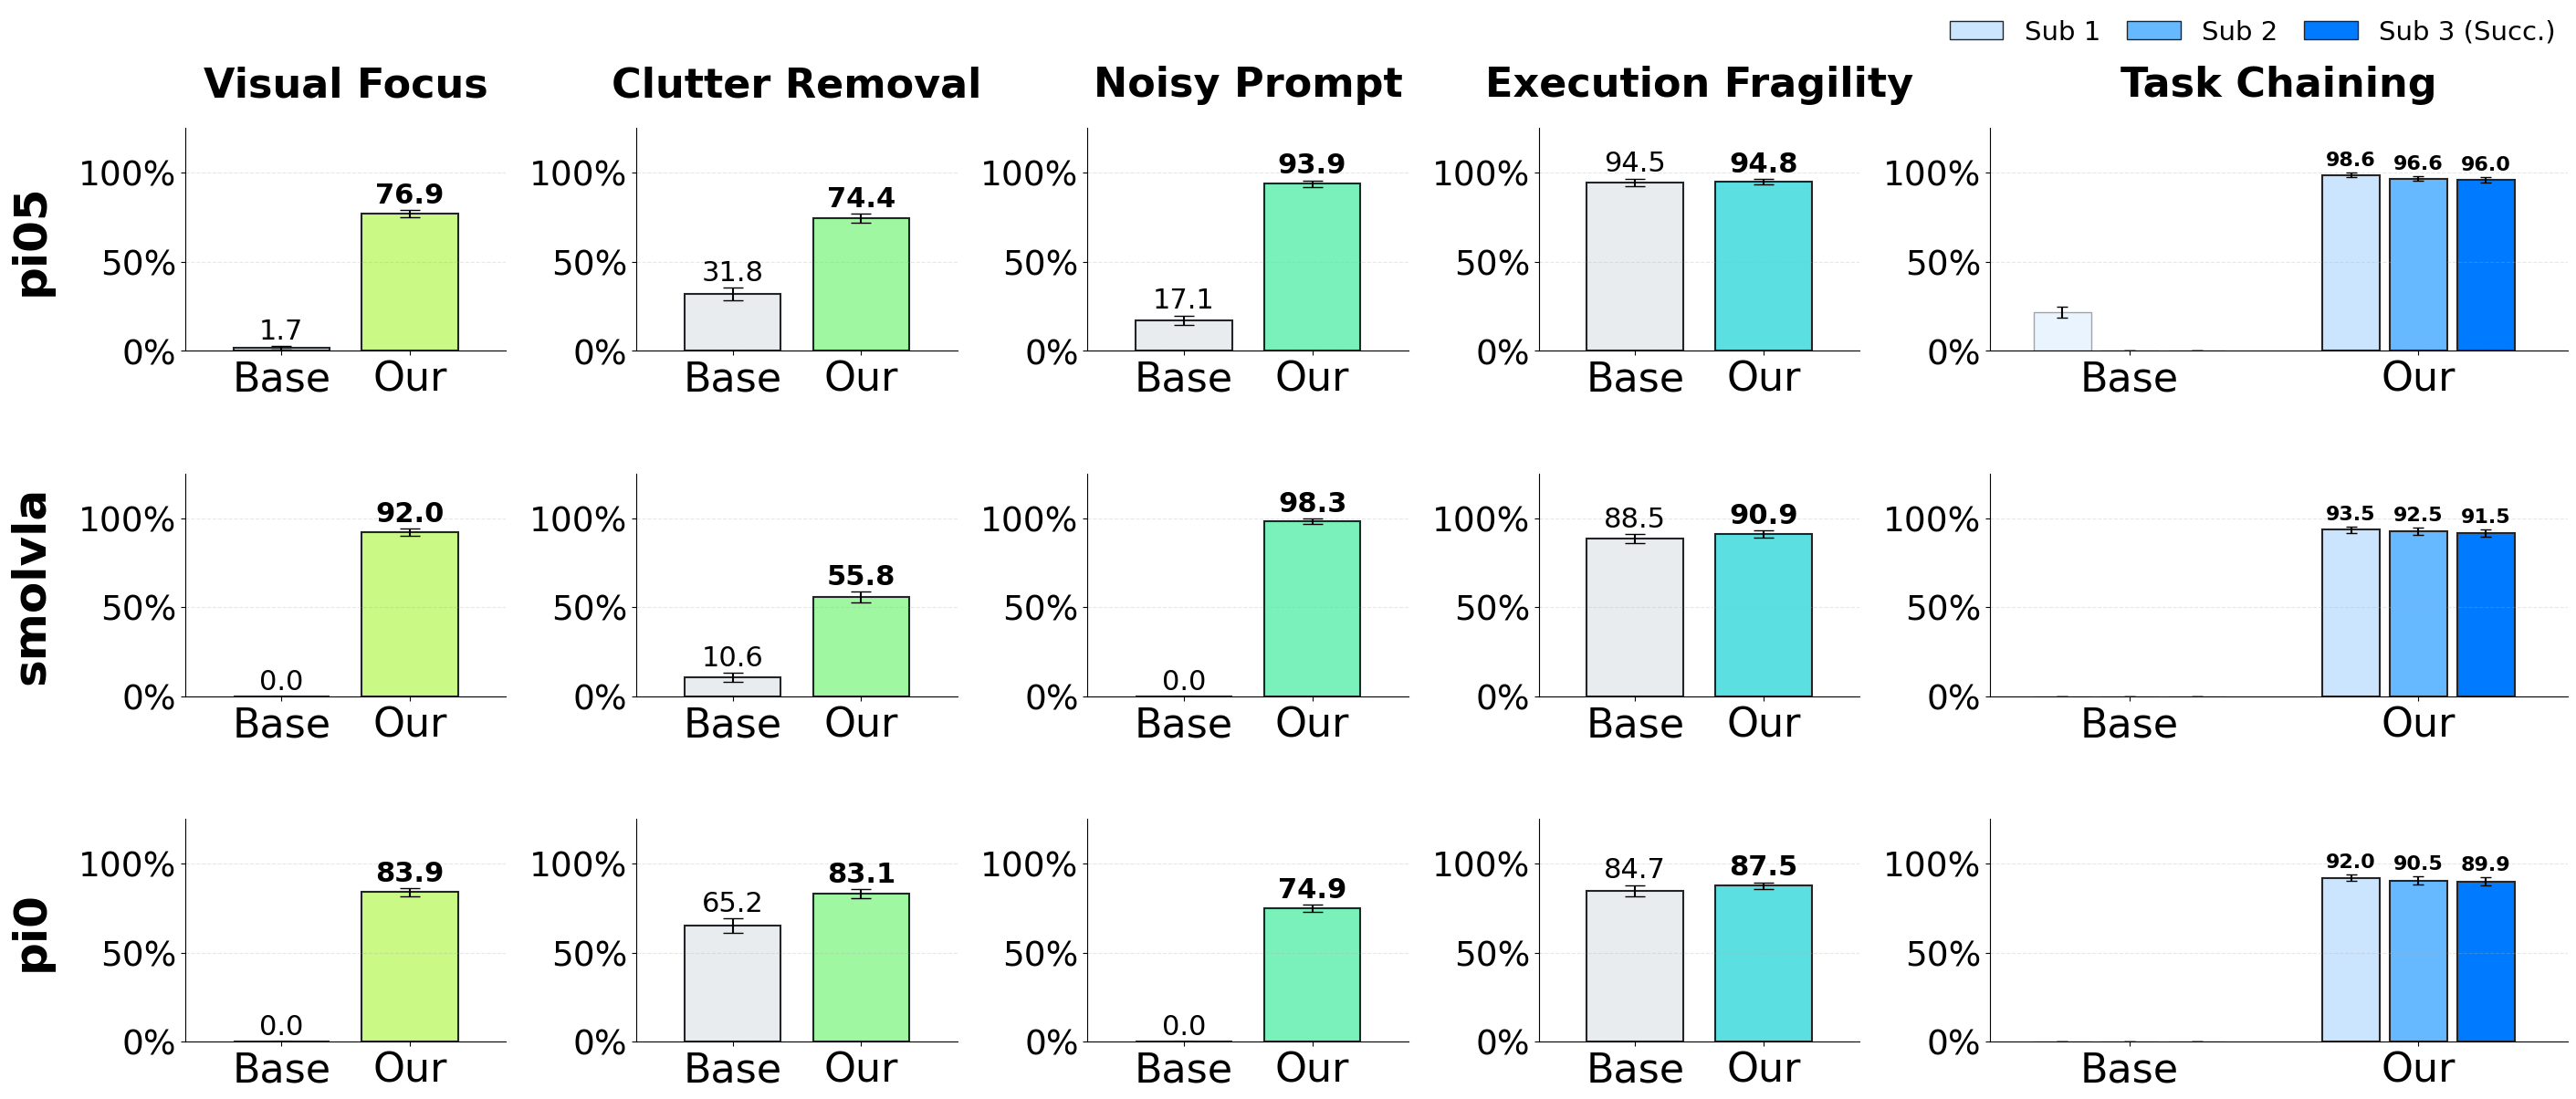
\includegraphics[width=\linewidth]{figure/result.png}
    \captionof{figure}{\textbf{Performance on LIBERO-{\sys}.} Comparison of {\sys} and VLA baselines across visual, linguistic, and long-horizon challenges.}%
    \label{fig:result}
  \end{minipage}%
  \hspace{0.01\textwidth}%
  \begin{minipage}[t]{0.30\textwidth}
    \vspace{0pt}
    \centering
    {\color{black}
    \vspace{0pt}
    \small
    \setlength{\tabcolsep}{3pt}
    \renewcommand{\arraystretch}{1.02}
    \begin{tabular}{@{}p{0.48\linewidth}lr@{}}
    \toprule
    \multicolumn{1}{@{}l}{\textbf{Component}} & & \textbf{ms/step} \\
    \midrule
    \multirow{2}{=}{Baseline rollout} & Mean & 15.31 \\
    & P95 & 15.98 \\
    \cmidrule(lr){1-3}
    \multirow{2}{=}{RAG retrieval} & Mean & 0.005 \\
    & P95 & 0.005 \\
    \cmidrule(lr){1-3}
    \multirow{2}{=}{VLM orchestration} & Mean & 7.20 \\
    & P95 & 8.65 \\
    \cmidrule(lr){1-3}
    \multirow{2}{=}{SAM3 + Overlay} & Mean & 0.16 \\
    & P95 & 0.16 \\
    \cmidrule(lr){1-3}
    \multirow{2}{=}{SAM3 + Remove} & Mean & 0.16 \\
    & P95 & 0.16 \\
    \bottomrule
    \end{tabular}
    \vspace{-0.3em}
    \captionsetup{justification=raggedright,singlelinecheck=false}
    \vspace{0.2em}
    \captionof{table}{\textbf{Runtime overhead.} Amortized over 1000 LIBERO steps.}
    \label{tab:runtime_overhead}
    \renewcommand{\arraystretch}{1.0}
    }
  \end{minipage}
  \vspace{-0.5em}
\end{figure*}

% \begin{table}[t] % 这里的 [t] 让它浮动到当前或后续页面的顶部
%   \centering
%   \caption{Success rates on LIBERO-PRO position tasks comparison between $\pi_{0.5}$ baseline and {\sys}-augmented policy.}
%   \label{tab:libero_pro_pos}
%   \small 
%   \addtolength{\tabcolsep}{-2pt} % 稍微压缩列间，使其在单栏内更紧凑
%   \begin{tabular}{@{}llcc@{}}
%     \toprule
%     & & \multicolumn{2}{c}{\textbf{LIBERO-PRO (Pos)}} \\ \cmidrule(l){3-4} 
%     \textbf{Category} & \textbf{Task (Symbolic Form)} & \textbf{Base} & \textbf{w/ {\sys}} \\ \midrule
    
%     % 第一组：Spatial-Swap
%     \multirow{5}{*}{\textbf{Spatial}} 
%     & $Pick(btw(p, r), plate)$        & 2\% & \textbf{63.00\%} \\
%     & $Pick(center, plate)$           & 0\% & \textbf{97.00\%} \\
%     & $Pick(drw_{top}(cab_{w}), plate)$ & 0\% & \textbf{20.20\%} \\
%     & $Pick(next\_to(p), plate)$      & 0\% & \textbf{57.00\%} \\
%     & $Pick(next\_to(r), plate)$      & 12\% & \textbf{71.00\%} \\
%     \cmidrule{2-4}
%     \multicolumn{2}{@{}l}{\textit{\textbf{Average}}} & 2.80\% & \textbf{61.64\%} \\
    
%     \midrule
%     % 第二组：Object-Swap
%     \textbf{Object} 
%     & $Pick(soup, basket)$            & 0\% & \textbf{35.00\%} \\
%     \cmidrule{2-4}
%     \multicolumn{2}{@{}l}{\textit{\textbf{Average}}}  & 0.00\% & \textbf{35.00\%} \\
%     \bottomrule
%   \end{tabular}
%   \vspace{-1.5em}
% \end{table}

% \begin{table}[t] % 这里的 [t] 让它浮动到当前或后续页面的顶部
%   \centering
%   \caption{Success rates on LIBERO-PRO task-level perturbed tasks comparison between $\pi_{0.5}$ baseline and {\sys}-augmented policy.}
%   \label{tab:libero_pro_task}
%   \small 
%   \addtolength{\tabcolsep}{-2pt} % 稍微压缩列间，使其在单栏内更紧凑
%   \begin{tabular}{@{}llcc@{}}
%     \toprule
%     & & \multicolumn{2}{c}{\textbf{LIBERO-PRO (Task)}} \\ \cmidrule(l){3-4} 
%     \textbf{Category} & \textbf{Task (Symbolic Form)} & \textbf{Base} & \textbf{w/ {\sys}} \\ \midrule
    
%     % 第一组：Spatial
%     \multirow{9}{*}{\textbf{Spatial}} 
%     & $Pick(btw(p, r), plate)$          & 0\% & \textbf{78.00\%} \\
%     & $Pick(center, plate)$             & 2\% & \textbf{82.00\%} \\
%     & $Pick(next\_to(cookie), plate)$   & 2\% & \textbf{97.00\%} \\
%     & $Pick(next\_to(p), plate)$        & 0\% & \textbf{73.00\%} \\
%     & $Pick(next\_to(r), plate)$        & 2\% & \textbf{98.00\%} \\
%     & $Pick(on(cookie), plate)$         & 0\% & \textbf{12.00\%} \\
%     & $Pick(on(r), plate)$              & 2\% & \textbf{100.00\%} \\
%     & $Pick(on(stove), plate)$          & 0\% & \textbf{13.00\%} \\
%     & $Pick(on(cab_{w}), plate)$        & 0\% & \textbf{95.00\%} \\
%     \cmidrule{2-4}
%     \multicolumn{2}{@{}l}{\textit{\textbf{Average}}} & 0.89\% & \textbf{72.00\%} \\
    
%     \midrule
%     % 第二组：Object
%     \multirow{5}{*}{\textbf{Object}} 
%     & $Pick(soup, basket)$              & 0\% & \textbf{16.00\%} \\
%     & $Pick(bbq, basket)$               & 2\% & \textbf{32.00\%} \\
%     & $Pick(juice, basket)$             & 2\% & \textbf{41.00\%} \\
%     & $Pick(dressing, basket)$          & 0\% & \textbf{13.00\%} \\
%     & $Pick(tomato, basket)$            & 0\% & \textbf{23.00\%} \\
%     \cmidrule{2-4}
%     \multicolumn{2}{@{}l}{\textit{\textbf{Average}}}  & 0.80\% & \textbf{25.00\%} \\
%     \bottomrule
%   \end{tabular}
% \end{table}


\begin{table}[t]
  \centering
\caption{\textbf{Performance on LIBERO-PRO.} Success rates under layout (Pos) and semantic (Task) shifts.}%
  \label{tab:libero_pro}
  \small % 调小字号至 footnotesize 以防止冲出栏宽
  \addtolength{\tabcolsep}{-4pt} % 极限压缩列间距
  
  {
  \setlength{\aboverulesep}{0pt}
  \setlength{\belowrulesep}{0pt}
  
  \begin{tabular}{l|clcc}
    \toprule
    \rule{0pt}{3ex} \textbf{Level} & \textbf{Category} & \textbf{Task (Symbolic Form)} & \textbf{$\pi_{0.5}$BASE} & \textbf{w/Our} \\
    \midrule
    
    % --- Position Level ---
    \rule{0pt}{2.5ex} \multirow{6}{*}{\textbf{Pos}} & \multirow{5}{*}{\textbf{Spat.}} 
      & $P.(btw(p, r), pl.)$        & 2\% & \textbf{63.0\%} \\
    & & $P.(center, pl.)$            & 0\% & \textbf{97.0\%} \\
    & & $P.(drw_{top}(cab_{w}), pl.)$ & 0\% & \textbf{20.2\%} \\
    & & $P.(next\_to(p), pl.)$       & 0\% & \textbf{57.0\%} \\
    & & $P.(next\_to(r), pl.)$       & 12\% & \textbf{71.0\%} \\
    \cmidrule(l){2-5}
    & \rule{0pt}{2.5ex} \textbf{Obj.} & $P.(soup, bskt.)$ & 0\% & \textbf{35.0\%} \\
    \midrule
    % 修复后的行：把 \rule 放在 \multicolumn 内部
    \multicolumn{3}{l|}{\rule{0pt}{2.5ex} \textit{\textbf{Average (Pos)}}} & 2.33\% & \textbf{57.2\%} \\
    
    \midrule 
    
    % --- Task Level ---
    \rule{0pt}{3ex} \multirow{14}{*}{\textbf{Task}} & \multirow{9}{*}{\textbf{Spat.}} 
      & $P.(btw(p, r), pl.)$          & 0\% & \textbf{78.0\%} \\
    & & $P.(center, pl.)$              & 2\% & \textbf{82.0\%} \\
    & & $P.(next\_to(ck.), pl.)$    & 2\% & \textbf{97.0\%} \\
    & & $P.(next\_to(p), pl.)$        & 0\% & \textbf{73.0\%} \\
    & & $P.(next\_to(r), pl.)$        & 2\% & \textbf{98.0\%} \\
    & & $P.(on(ck.), pl.)$          & 0\% & \textbf{12.0\%} \\
    & & $P.(on(r), pl.)$               & 2\% & \textbf{100.0\%} \\
    & & $P.(on(stove), pl.)$           & 0\% & \textbf{13.0\%} \\
    & & $P.(on(cab_{w}), pl.)$        & 0\% & \textbf{95.0\%} \\
    \cmidrule(l){2-5}
    & \rule{0pt}{2.5ex} \multirow{5}{*}{\textbf{Obj.}} 
      & $P.(soup, bskt.)$              & 0\% & \textbf{16.0\%} \\
    & & $P.(bbq, bskt.)$               & 2\% & \textbf{32.0\%} \\
    & & $P.(juice, bskt.)$             & 2\% & \textbf{41.0\%} \\
    & & $P.(dressing, bskt.)$          & 0\% & \textbf{13.0\%} \\
    & & $P.(tomato, bskt.)$            & 0\% & \textbf{23.0\%} \\
    \midrule
    % 同理修复
    \multicolumn{3}{l|}{\rule{0pt}{2.5ex} \textit{\textbf{Average (Task)}}} & 0.86\% & \textbf{55.2\%} \\
    \bottomrule
  \end{tabular}
  }
  \vspace{-1.5em}
\end{table}
We evaluate {\sys} across multiple foundation models on 25 tasks. We further conduct ablation studies to validate the Dual-Stage Memory Consolidation mechanism.
Results show that {\sys} consistently improves in-context adaptation and policy robustness across scenarios.

To improve statistical reliability under real-robot cost and trial constraints, we prioritize rigorous testing in a high-fidelity simulation environment.

\subsection{Experimental Setup}
\noindent\textbf{Task Design and Evaluation Benchmarks.}
To evaluate robust in-context adaptation under distribution shifts, we conduct experiments across two task suites. We first adopt the \textbf{LIBERO-PRO}~\cite{liberopro} benchmark to test robustness against Position-swap (LIBERO-PRO Pos) and Task-level (LIBERO-PRO Task) variations within Spatial and Object categories.

Furthermore, we introduce \textbf{LIBERO-{\sys}}. This suite formalizes five \textit{prevalent and critical} OOD challenge dimensions across simulated and real-world robotics. By reconfiguring assets within LIBERO scenarios~\cite{libero_ref}, it provides a controlled environment to assess an agent's ability to trigger adaptive interventions for recurring failure modes without task-specific fine-tuning.


\begin{itemize}
    \item \textbf{Visual Focus}: Selecting a target from five identical, novel bowls. By substituting \textit{LIBERO-Spatial} targets with indistinguishable assets, we evaluate \textbf{referential grounding} under fine-grained visual ambiguity.

    \item \textbf{Clutter Removal}: Grasping targets amidst dense distractors. We augment \textit{LIBERO-Spatial} with high-entropy object clusters to test \textbf{operational focus} and interference mitigation in crowded scenes.

    \item \textbf{Noisy Prompt}: {\color{black}Intent extraction from instructions whose wording or task structure deviates from historical successful experience patterns} (e.g., \textit{``Umm\ldots get that red squeezy thing''}). By injecting linguistic noise into \textit{LIBERO-Object} instructions, we assess \textbf{linguistic robustness} and {\color{black}experience-grounded semantic mapping}.

    \item \textbf{Execution Fragility}: Critical maneuvers where minor slips trigger failure. We curate unstable sub-tasks from \textit{LIBERO-Object} to evaluate \textbf{operational stability} against mechanical uncertainties.

    \item \textbf{Task Chaining}: Long-horizon sorting of multiple objects into a basket. By sequencing atomic \textit{LIBERO-Object} actions, this task evaluates \textbf{long-term reasoning} and \textbf{error resilience} in sequential workflows.
\end{itemize}

% \noindent\textbf{Complex Spatial and Object Reasoning.}
% Beyond the aforementioned OOD challenges, we further evaluate the model on the \textbf{LIBERO-PRO}~\cite{liberopro} benchmark, testing its robustness against Position-swap (\textbf{Pos}) and Task-level (\textbf{Task}) variations within \textbf{Spatial} and \textbf{Object} tasks. 

\noindent\textbf{In-Context Initialization and Metrics.}
We initialize Dual-Memory RAG with a preliminary inference pass on standard LIBERO-Object and LIBERO-Spatial sets.
This non-parametric ``cold start'' populates the memory bank with generic execution traces, without gradient-based training or exposure to evaluation-time OOD perturbations.
We then run 199 randomized rollouts per task, fully shuffling object poses and task sequences to reduce bias.
Performance is measured by \textbf{overall completion rates} and \textbf{intermediate success rates} for granular long-horizon analysis.

\noindent\textbf{Baselines.}
We evaluate {\sys} on diverse foundation models, including $\pi_0$~\cite{pi0}, $\pi_{0.5}$~\cite{pi05}, and SmolVLA~\cite{SmolVLA}.
Across OOD scenarios, {\sys} consistently improves success rates, indicating better policy generalization.

\subsection{Main Results}%
\label{Main Results}

% \begin{figure*}[t]
%   \centering
%   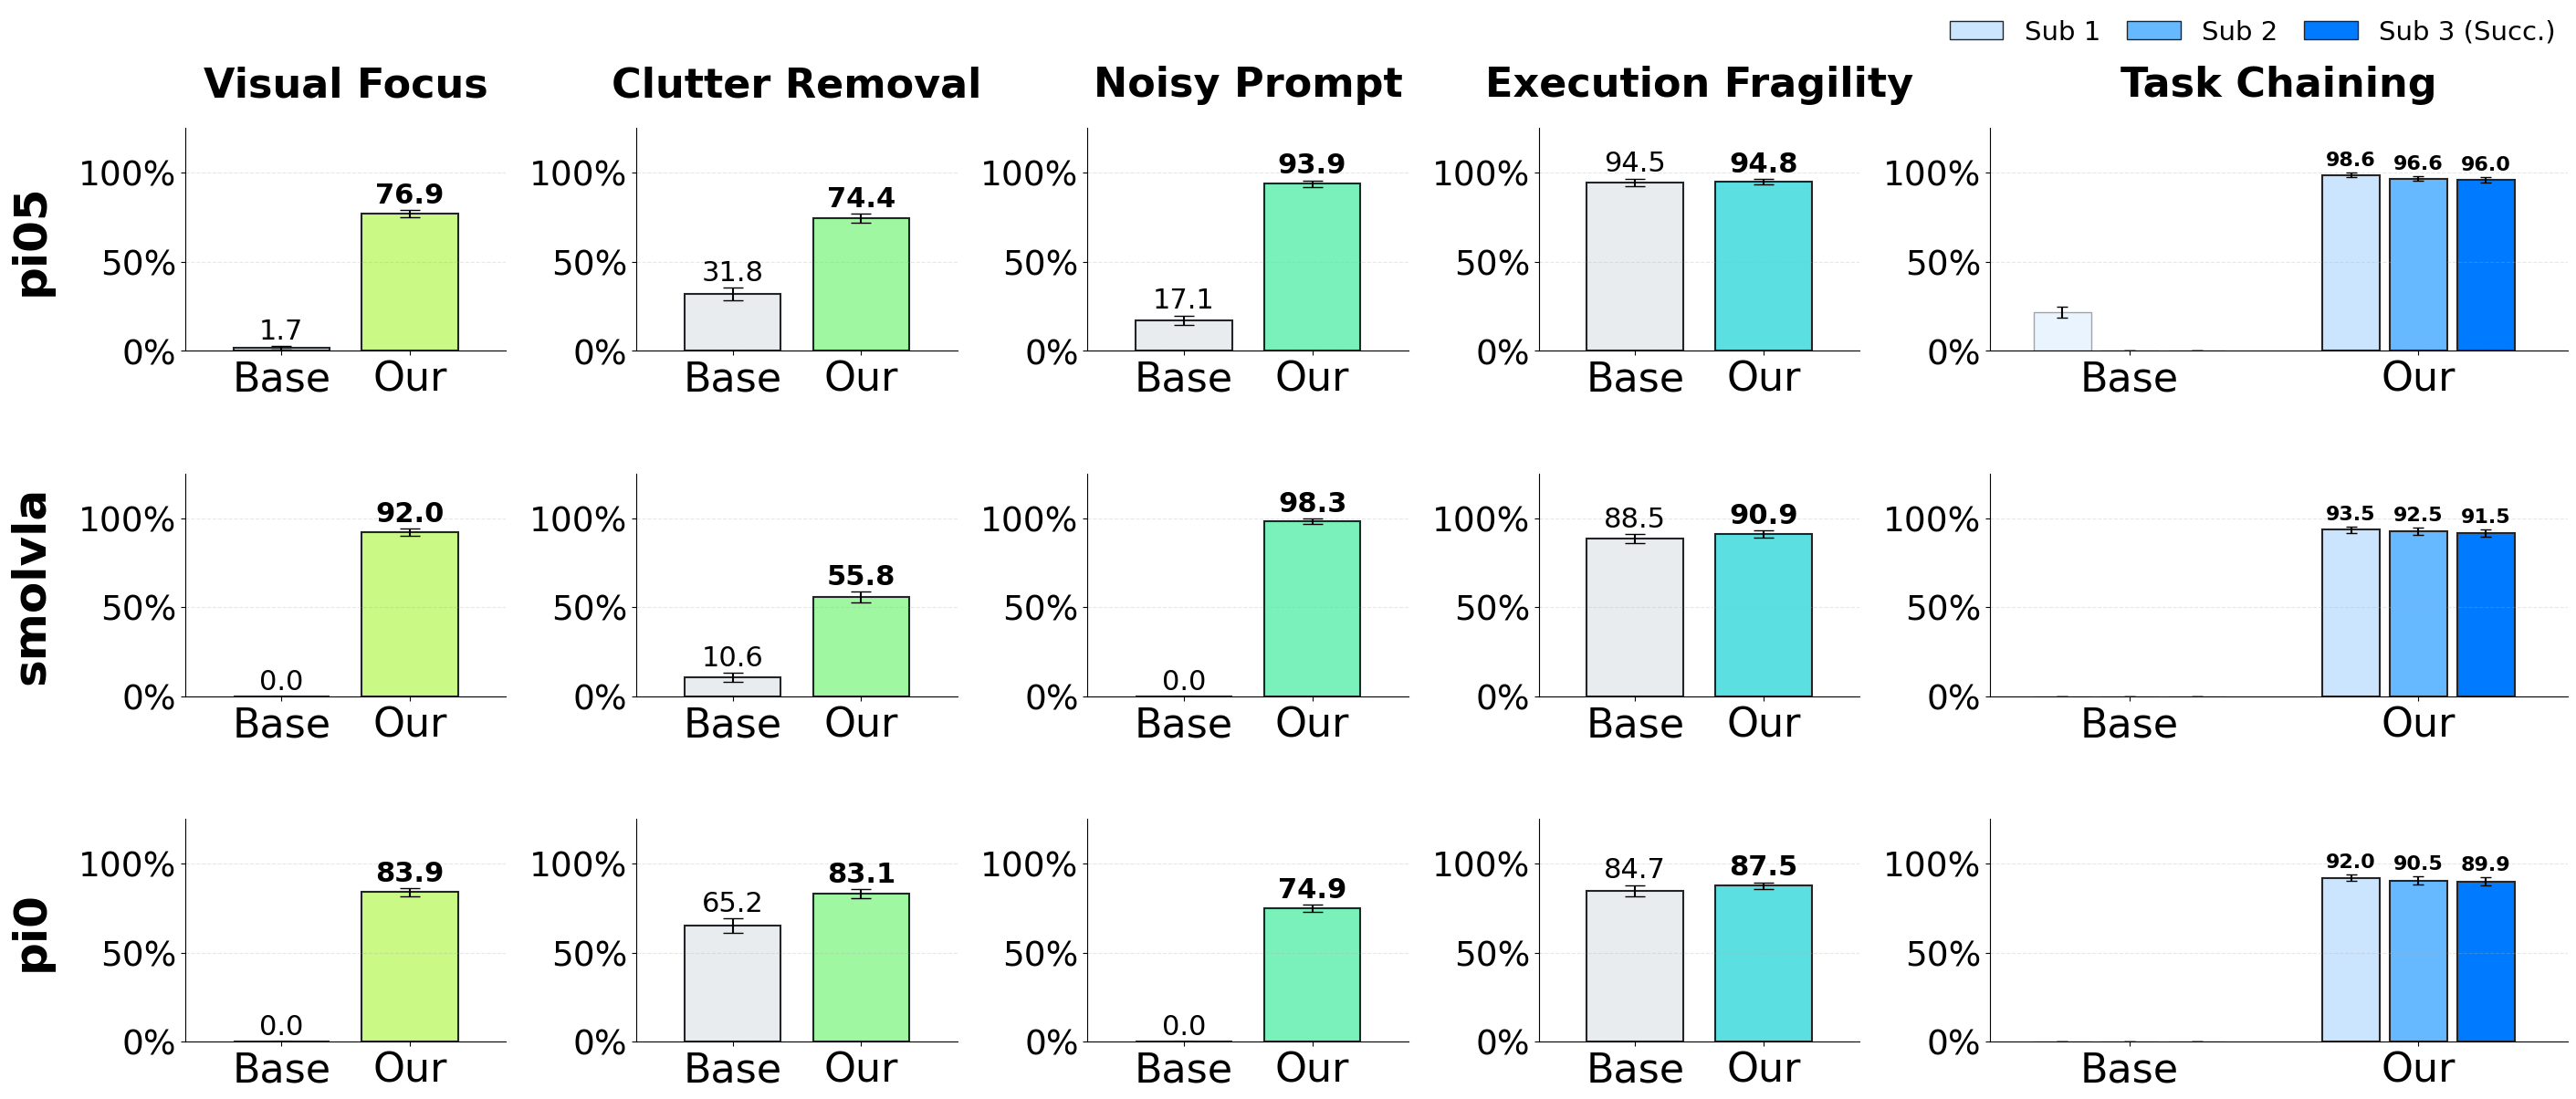
\includegraphics[width=0.8\linewidth]{figure/result.png}
%     \caption{\textbf{Performance comparison of {\sys} across diverse robotic foundation models and OOD challenges.} The results demonstrate that {\sys} consistently yields substantial performance gains for all base models across visual, linguistic, and long-horizon tasks.}
%   \label{fig:result}
% \end{figure*}
As shown in Fig.~\ref{fig:result} and Table~\ref{tab:libero_pro}, {\sys}-augmented policies improve robustness on both LIBERO-{\sys} and LIBERO-PRO, especially under perceptual ambiguity, linguistic noise, and long-horizon compounding errors.

\subsubsection{Results on LIBERO-{\sys}}

\noindent\textbf{Environmental and Linguistic Variations.}
Base models are sensitive to sensory and linguistic interference.
For \textit{pi05-LIBERO}, \textit{Visual Focus} and \textit{Clutter Removal} success rates increase from $1.7\%$ and $31.8\%$ to $76.9\%$ and $74.4\%$ with {\sys}, showing MCP-based interventions help isolate task-relevant objects.
For language perturbations, \textit{smolvla-LIBERO} reaches $98.3\%$ on \textit{Noisy Prompt} after instruction refinement.

\noindent\textbf{Execution Stability and Long-Horizon Tasks.}
In \textit{Execution Fragility}, {\sys} raises success rates above $87\%$ for all models by adding recovery-oriented interventions.
{\color{black}Since the baseline success rates in \textit{Execution Fragility} are already relatively high, {\sys}'s improvement is smaller in absolute terms and mainly comes from reducing the remaining rare failures through rollback and retry.}
In \textit{Task Chaining}, {\sys} reduces compounding errors through subtask decomposition and control-flow reset; notably, \textit{pi05-LIBERO} maintains $96.0\%$ success through the final sub-task.


\subsubsection{Results on LIBERO-PRO}

\noindent\textbf{Position-Level Layout Shifts.}
Under LIBERO-PRO Pos, the $\pi_{0.5}$ baseline achieves only $2.33\%$ average success, while {\sys} improves it to $57.2\%$.
{\color{black}This suggests that memory-guided visual interventions help recover object grounding under layout shifts.}

\noindent\textbf{Task-Level Semantic Perturbations.}
Under LIBERO-PRO Task, the baseline averages only $0.86\%$ success, whereas {\sys} reaches $55.2\%$.
{\color{black}These gains indicate that {\sys} improves the input and task context for the frozen controller, rather than replacing the low-level VLA policy.}

{\color{black}
\subsubsection{Discussion}
The large gains stem from compensating for frozen VLAs' statelessness under OOD layouts, distractors, noisy prompts, and long-horizon chains.
{\sys} retrieves success/failure memories to diagnose failures and trigger task-level MCP interventions before execution.
}

{\color{black}
\subsubsection{Online Latency}
Table~\ref{tab:runtime_overhead} reports latency amortized over a 1000-step LIBERO task, with baseline rollout measured on an RTX 4090.
RAG retrieval and SAM3-based tools add negligible amortized overhead, while VLM orchestration is the main extra cost.
Because {\sys} invokes these modules before rollout rather than at every policy step, low-level execution remains smooth and non-blocking.
In pipelined multi-task settings, next-task orchestration can overlap with current task execution.
}





% \begin{table*}[t]
% \centering
% % --- 标题与标签 ---
% \caption{\textbf{Ablation Study:} Comparison of reasoning logic and success rates across RAG configurations.}%
% \label{ablation}
% % ------------------
% \footnotesize 
% \begin{tabularx}{\textwidth}{|M{1.8cm}|X|M{3.5cm}|M{2.1cm}|M{1.8cm}|M{1.1cm}|}
% \hline
% \textbf{RAG Config} & \multicolumn{1}{c|}{\textbf{Reasoning}} & \textbf{MCP Tool} & \textbf{Action Result} & \textbf{Task Image} & \textbf{SR (\%)} \\ \hline

% % --- No RAG ---
% \multirow{3}{*}{No-RAG} & Ambiguity in target ID due to identical textures. & $o_t' = \text{Paint-to-Action}(o_t, \theta_{\text{dist}})$ & Highlight bowl & \multirow{3}{*}{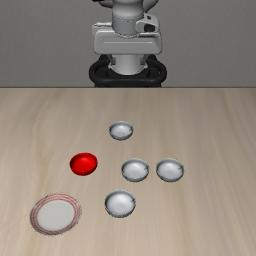
\includegraphics[width=0.95cm, valign=m]{figure/no_origin.jpg}} & \multirow{3}{*}{19.2} \\ \cline{2-4}
%  & Potential detection errors from plate shadows. & \texttt{none} & --- & & \\ \cline{2-4}
%  & Clean background, no distractors found. & \texttt{none} & --- & & \\ \hline

% % --- Limited RAG ---
% \multirow{4}{*}{Limited-RAG} & Edge proximity causes occlusion; highlight target. & $o_t' = \text{Paint-to-Action}(o_t, \theta_{\text{dist}})$ & Highlight bowl & \multirow{4}{*}{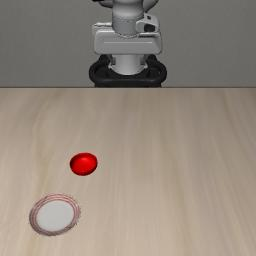
\includegraphics[width=0.95cm, valign=m]{figure/limit_origin.jpg}} & \multirow{4}{*}{48.8} \\ \cline{2-4}
%  & 1. \textbf{Past failures} suggest high mis-ID risk. & \multirow{2}{*}{$o_t'' = \text{Eraser}(o_t', \theta_{\text{conf}})$} & \multirow{2}{*}{Remove 4 dist.} & & \\ 
%  & 2. Focus by \textbf{removing} identical distractors. & & & & \\ \cline{2-4}
%  & \textbf{Background replace} to reduce visual noise. & $o_t''' = \text{Eraser}(o_t'', \theta_{\text{conf}})$ & BG Replacement & & \\ \hline

% % --- Rich RAG ---
% \multirow{5}{*}{Rich-RAG} & 1. High risk from \textbf{distractors via failure memory}. & \multirow{4}{*}{$o_t' = \text{Eraser}(o_t, \theta_{\text{conf}})$} & \multirow{4}{*}{Remove 4 dist.} & \multirow{5}{*}{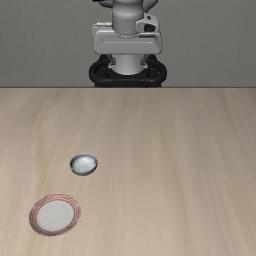
\includegraphics[width=0.95cm, valign=m]{figure/rich_origin.jpg}} & \multirow{5}{*}{60.1} \\ 
%  & 2. \textbf{Memory} dictates explicit removal of each bowl. & & & & \\ 
%  & 3. Strategic preservation of target and plate. & & & & \\ 
%  & 4. Use precise position to guide policy. & & & & \\ \cline{2-4}
%  & \textbf{Distraction-free; no visual overlay needed.} & \texttt{none} & -- & & \\ \hline

% \end{tabularx}
% \end{table*}



% \begin{figure}[htbp]
%      \centering
%      % 调整了图片宽度，单张图通常建议设置在 0.6\textwidth 到 0.8\textwidth 之间
%      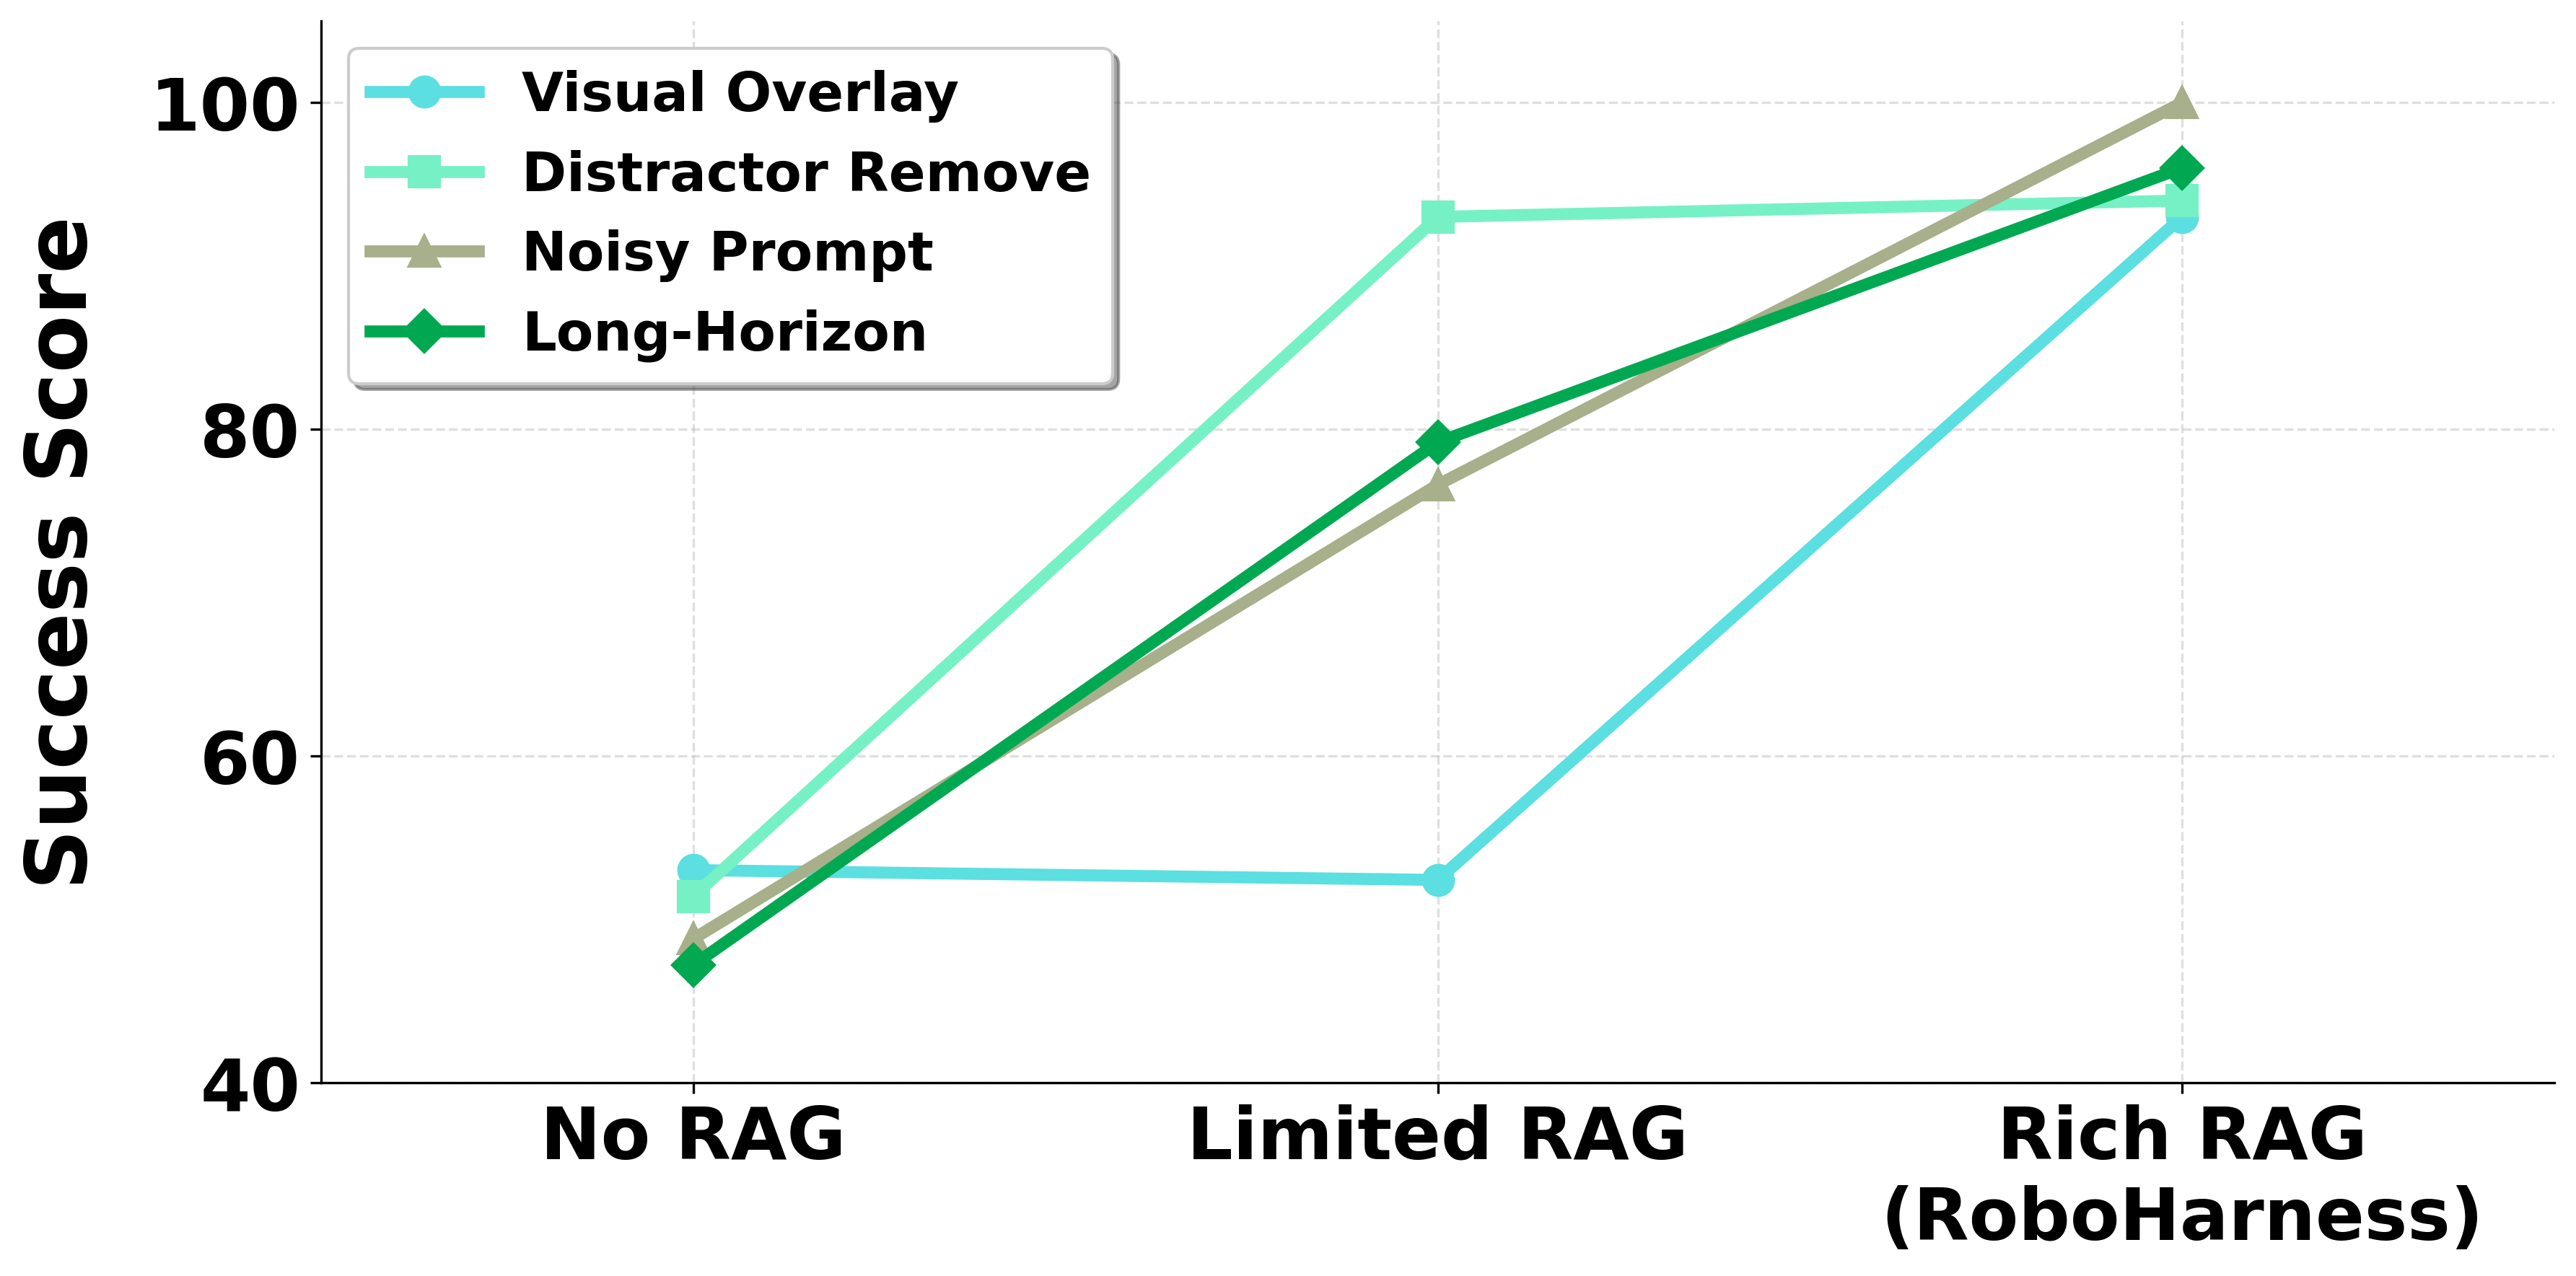
\includegraphics[width=0.45\textwidth]{figure/ablation2.png}
     
%      % 更新了主标题，去除了对(a)(b)的引用，直接描述该图内容
%     \caption{\textbf{Ablation Study:} Evolution of qualitative reasoning depth scores across configurations.}%
%     \label{score_qwen} 
%      % 保留原主标签，或者如果你更习惯用之前的子标签 \label{score_qwen} 也可以替换
% \end{figure}

% \noindent\textbf{Quantitative Performance and Stability}
% We evaluate our framework on a variant of the ``Clutter Removal'' task using Pi-0.5 as the base policy.
% As shown in Table~\ref{ablation}, success rates scale with the richness of RAG information.
% The No RAG baseline yields only 19.20\%; notably, comparison with Section~\ref{Main Results} suggests that relying solely on LLM guidance without RAG can even be counterproductive, potentially introducing negative biases.
% Performance improves to 48.80\% with Limited RAG, though its tool chain reveals a reliance on redundant steps like unnecessary background replacement.
% In contrast, Rich RAG ({\sys}) achieves a peak success rate of 60.10\% through a streamlined reasoning chain, demonstrating superior strategic efficiency and precision.


% \noindent\textbf{Qualitative Evaluation of Reasoning Depth}
% To assess the model's cognitive depth, we use Qwen3-VL-32B to score the logical coherence of generated instructions.
% As illustrated in Fig.~\ref{score_qwen}, Rich RAG consistently secures the highest ratings across all dimensions.
% This advantage stems from optimized reasoning trajectories that prioritize critical intervention points, thereby reducing ineffective action sequences.
% These results indicate that high-quality RAG data directly strengthens the model's grasp of task causality, forming a more robust tool-invocation chain that aligns with the observed quantitative gains.



\subsection{Ablation Study}

With the {\color{black}orchestrator + MCP modules} validated in Section~\ref{Main Results}, we further analyze the \textbf{Dual} design of our Dual-Memory RAG system. Following Section~\ref{dual memory ablation}, we proceed in two steps: we first isolate the Dual-Memory Bank's effect on execution efficiency, then evaluate the contribution of Dual-Stage Memory Consolidation to reasoning depth.

\subsubsection{Efficacy of the Dual-Memory Bank}%
\label{dual memory ablation}
To verify the need for both successful and failed experiences in anchoring {\color{black}orchestrator decisions}, we use Average Turns-to-Success~\cite{multiwoz,toolsandbox}, which measures the number of reasoning-intervention loops required to reach an optimal plan.
When an intervention fails, the agent receives sparse environmental feedback and must self-correct in subsequent turns.
As shown in Fig.~\ref{fig:ablation_beeswarm}, we compare four memory configurations: \textbf{No Memory}, \textbf{Failure Only}, \textbf{Success Only}, and \textbf{{\sys} (Dual)}.

\begin{figure}[htbp]
   \vspace{0.5em}
    \centering
    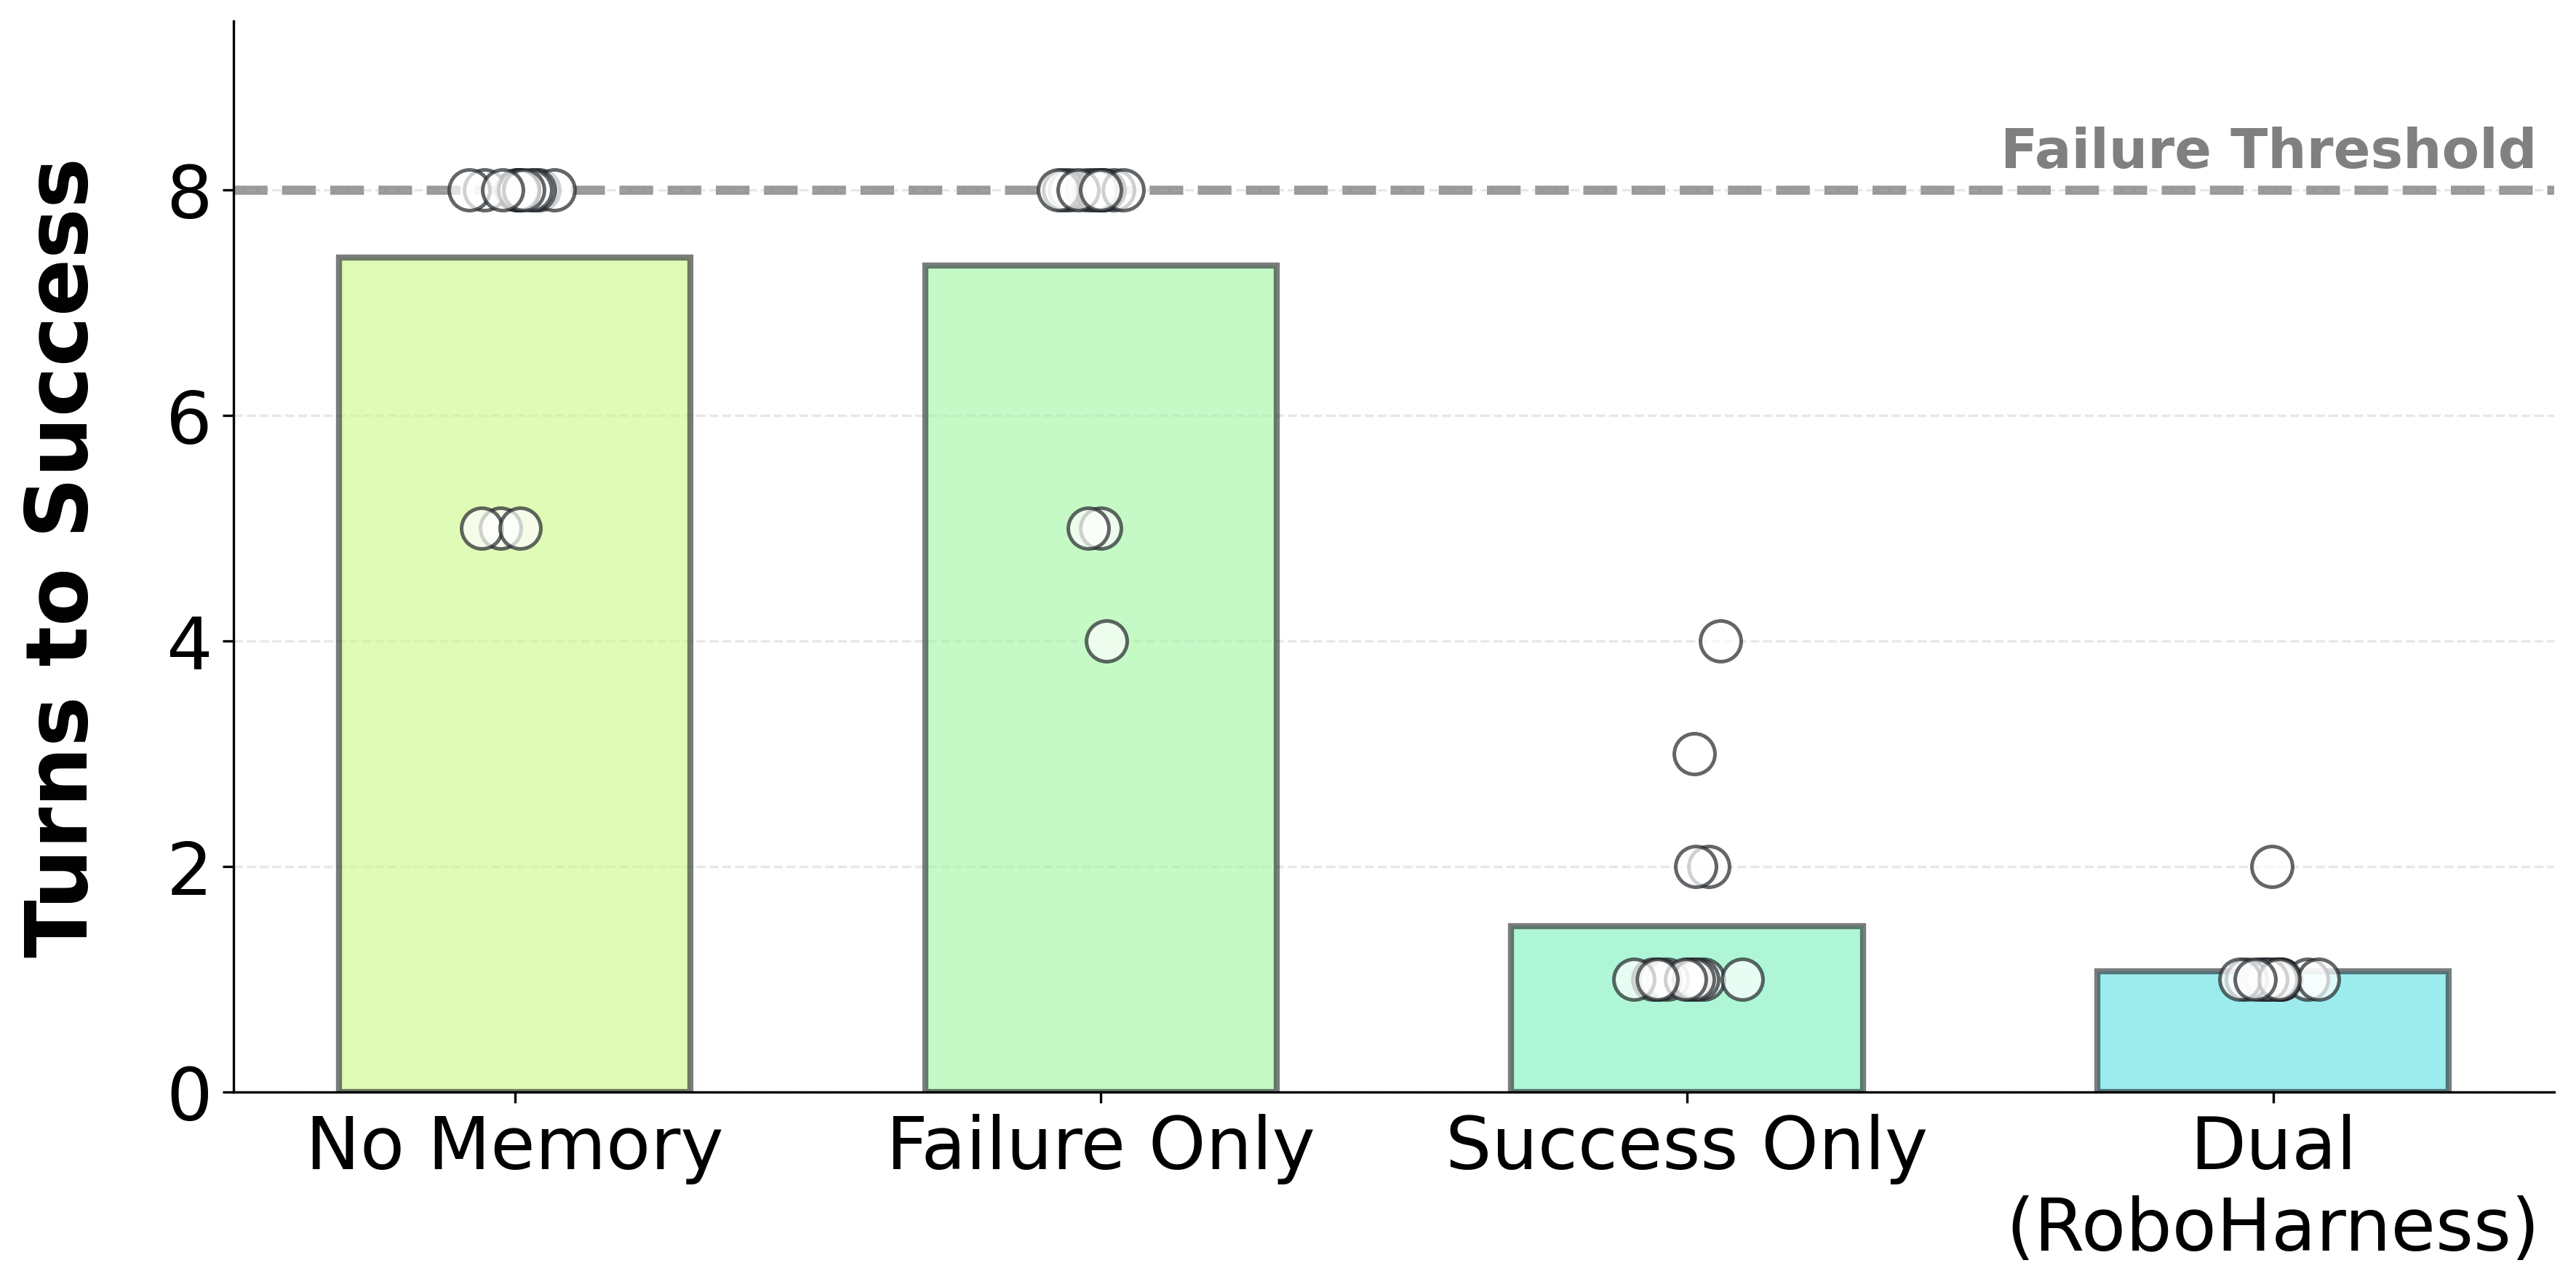
\includegraphics[width=0.4\textwidth]{figure/ablation_dual_memory.png}
    \caption{\textbf{Ablation Study.} Distribution of reasoning turns required to reach the target intervention plan.}%
    \label{fig:ablation_beeswarm}
    \vspace{-0.5em}

\end{figure}

As shown in Fig.~\ref{fig:ablation_beeswarm}, the baseline without memory consistently reaches the maximum execution timeout ($Mean = 7.40$), indicating that zero-shot reasoning is insufficient for OOD recovery. While \textit{Success-Only} memory reduces the average turns to $1.47$, it still exhibits significant stochastic variance. In contrast, \textbf{{\sys} (Dual)} converges to a near-optimal \textbf{$1.07$} turns. The dual-memory bank constrains the search space for the {\color{black}vision-language orchestrator}, enabling directed decision-making instead of stochastic exploration.

\subsubsection{Impact of Dual-Stage Memory Consolidation} 
While the dual-memory bank provides the raw data, the quality of these experiences is governed by the iterative attribution module described in Section~\ref{Evolution}. We evaluate this process via three configurations: \textbf{No RAG} (baseline), \textbf{Limited RAG} (single-stage online attribution), and \textbf{Rich RAG} ({\sys}'s dual-stage consolidation).

% --- Table Configuration ---
\newcolumntype{M}[1]{>{\centering\arraybackslash}m{#1}}
\renewcommand{\arraystretch}{1.1}
\setlength{\tabcolsep}{3pt}

\begin{table*}[t]
\vspace{0.5em}
\centering
\caption{\textbf{Ablation Study.} Comparison of reasoning logic and success rates across RAG configurations.}%
\label{ablation}
\footnotesize 
\begin{tabularx}{\textwidth}{|M{1.8cm}|X|M{3.5cm}|M{2.1cm}|M{1.8cm}|M{1.1cm}|}
\hline
\textbf{RAG Config} & \multicolumn{1}{c|}{\textbf{{\color{black}Orchestrator Reasoning via RAG}}} & \textbf{MCP Tool} & \textbf{Action Result} & \textbf{Task Image} & \textbf{SR (\%)} \\ \hline
\multirow{3}{*}{No-RAG} & Ambiguity in target ID due to identical textures. & $o_t' = \text{Paint-to-Action}(o_t, \theta_{\text{dist}})$ & Highlight bowl & \multirow{3}{*}{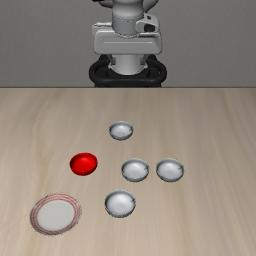
\includegraphics[width=0.95cm, valign=m]{figure/no_origin.jpg}} & \multirow{3}{*}{19.2} \\ \cline{2-4}
 & Potential detection errors from plate shadows. & \texttt{none} & --- & & \\ \cline{2-4}
 & Clean background, no distractors found. & \texttt{none} & --- & & \\ \hline
\multirow{4}{*}{Limited-RAG} & Edge proximity causes occlusion; highlight target. & $o_t' = \text{Paint-to-Action}(o_t, \theta_{\text{dist}})$ & Highlight bowl & \multirow{4}{*}{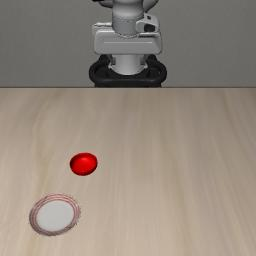
\includegraphics[width=0.95cm, valign=m]{figure/limit_origin.jpg}} & \multirow{4}{*}{48.8} \\ \cline{2-4}
 & 1. \textbf{Past failures} suggest high mis-ID risk. & \multirow{2}{*}{$o_t'' = \text{Eraser}(o_t', \theta_{\text{conf}})$} & \multirow{2}{*}{Remove 4 dist.} & & \\ 
 & 2. Focus by \textbf{removing} identical distractors. & & & & \\ \cline{2-4}
 & \textbf{Background replace} to reduce visual noise. & $o_t''' = \text{Eraser}(o_t'', \theta_{\text{conf}})$ & BG Replacement & & \\ \hline
\multirow{5}{*}{Rich-RAG} & 1. High risk from \textbf{distractors via failure memory}. & \multirow{4}{*}{$o_t' = \text{Eraser}(o_t, \theta_{\text{conf}})$} & \multirow{4}{*}{Remove 4 dist.} & \multirow{5}{*}{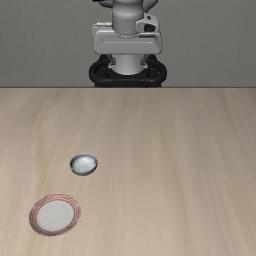
\includegraphics[width=0.95cm, valign=m]{figure/rich_origin.jpg}} & \multirow{5}{*}{60.1} \\ 
 & 2. \textbf{Memory} dictates explicit removal of each bowl. & & & & \\ 
 & 3. Strategic preservation of target and plate. & & & & \\ 
 & 4. Use precise position to guide policy. & & & & \\ \cline{2-4}
 & \textbf{Distraction-free; no visual overlay needed.} & \texttt{none} & --- & & \\ \hline
\end{tabularx}

\end{table*}

\begin{figure}[htbp]

     \centering
     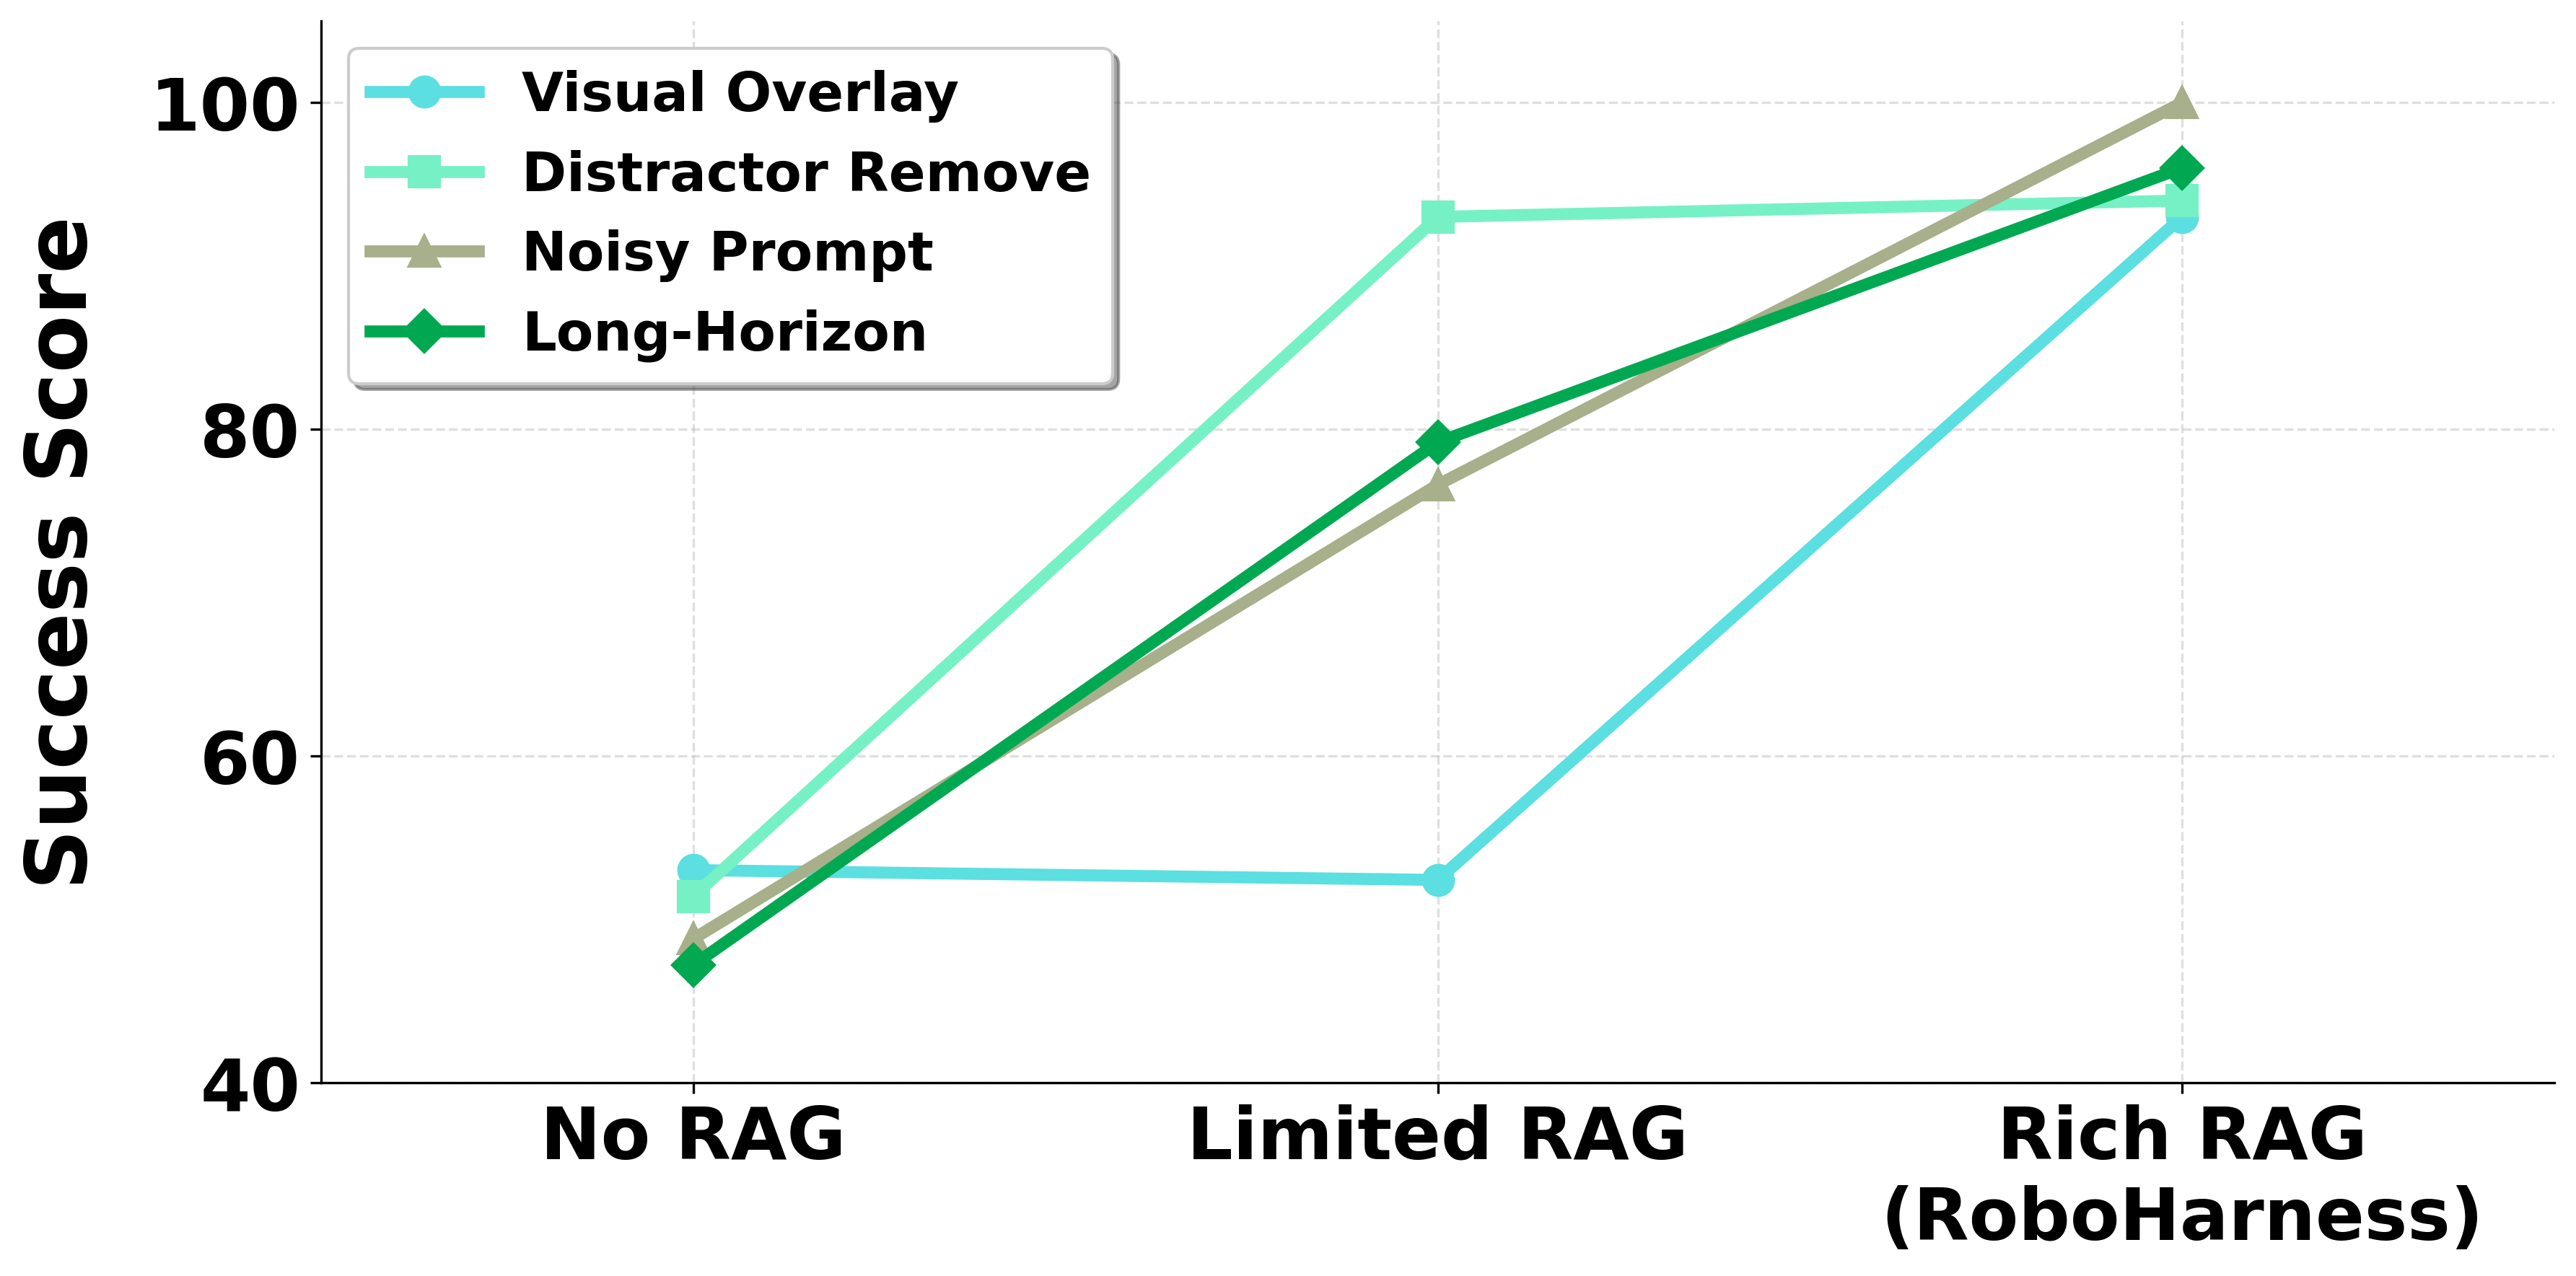
\includegraphics[width=0.4\textwidth]{figure/ablation2.png}
    \caption{\textbf{Ablation Study.} Evolution of qualitative reasoning depth scores across configurations.}%
    \label{score_qwen} 

\end{figure}


\noindent\textbf{Qualitative Evaluation of Reasoning Depth.}
We use Qwen3-VL-32B to score the logical coherence of generated instructions.
As shown in Fig.~\ref{score_qwen}, Rich RAG consistently achieves the highest ratings across all dimensions.
This gain comes from more focused reasoning trajectories that prioritize critical intervention points and reduce ineffective actions.
These results suggest that higher-quality RAG data improves causal understanding and yields a more robust tool-invocation chain, consistent with the quantitative gains.


\noindent\textbf{Quantitative Performance and Stability.}
We evaluate a ``Clutter Removal'' variant with $\pi_{0.5}$.
As shown in Table~\ref{ablation}, success rates increase with RAG richness.
No RAG achieves only $19.20\%$, and comparison with Section~\ref{Main Results} shows that {\color{black}orchestrator guidance} without RAG can be counterproductive by introducing negative bias.
Limited RAG improves performance to $48.80\%$ but still relies on redundant steps (e.g., unnecessary background replacement).
Rich RAG ({\sys}) reaches $60.10\%$ with a streamlined reasoning chain, showing higher strategic efficiency and precision.
